\begin{figure*}[t]
  \centering
  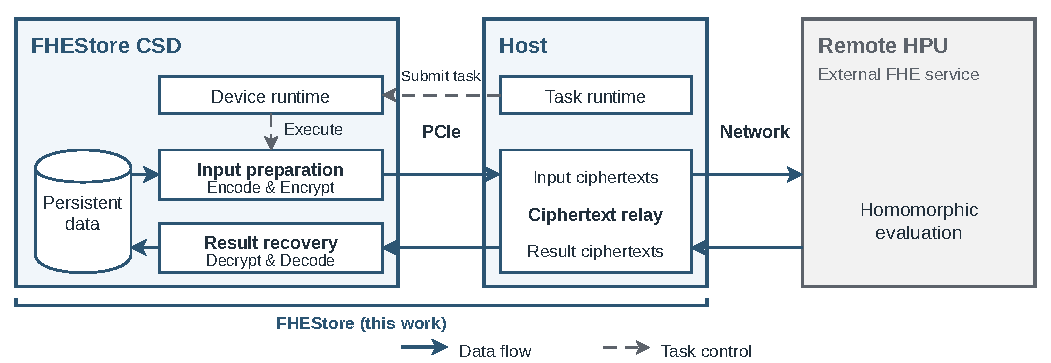
\includegraphics[width=\textwidth]{figures/fhestore-overview-v4/fhestore-overview.pdf}
  \caption{FHEStore comprises the CSD and host (blue), connected by PCIe; the remote HPU (gray) is an external service reached through the host over a network. Solid arrows denote logical data flow, and dashed arrows denote task control. Input preparation includes optional preprocessing, encoding, and encryption; result recovery includes decryption, decoding, and write-back, with host-assisted record merging where needed.}
  \Description{Three aligned regions show the CSD and host with blue borders and the external remote HPU with a gray border. A bracket identifies the CSD and host as FHEStore. The host task runtime submits tasks over PCIe to the device runtime. Persistent data flows through input preparation and the host ciphertext relay to the remote HPU over a network. Result ciphertexts return through the same host relay to device result recovery and storage.}
  \label{fig:fhestore-overview}
\end{figure*}
